\documentclass[12pt]{article}

\usepackage[a4paper, margin=2.5cm]{geometry}
\usepackage{graphicx}
\usepackage[T1]{fontenc}
\usepackage[utf8]{inputenc}
\usepackage{setspace}
\usepackage{booktabs}
\usepackage{caption}
\usepackage{subcaption}
\usepackage{amsmath}
\usepackage{hyperref}
\usepackage{circuitikz}
\usepackage{enumitem}
\usepackage{float}
\usepackage{pgfplots}
\pgfplotsset{compat=1.18}

\begin{document}

\begin{titlepage}
    \centering

    % University logo
    
\includegraphics[width=0.45\textwidth]{images/ozu_logo.png}\\[3cm]

    % Course
    {\large \textbf{EE 493 -- Power Electronics}}\\[1cm]

    % Semester
    {\large \textbf{Spring 2025/26}}\\[1cm]

    % Lab number
    {\large \textbf{TERM PROJECT}}\\[1cm]

    % Lab title
    {\large \textbf{Design of an Isolated Flyback DC-DC Converter}}\\[5cm]

    % Submission info
    \begin{center}
        {\normalsize \textbf{Submitted by:} Ömer Faruk AVCI}\\[0.4cm]
        {\normalsize \textbf{Student ID:} S034113}\\[0.4cm]
        {\normalsize \textbf{Date of Submission:} \today}
    \end{center}

\end{titlepage}

%------------------------------
% Introduction
%------------------------------
\section*{1 Introduction}
This term project covers the design, calculation, and simulation of a DC-DC Flyback converter operating over the 300V to 500V input range. The converter needs to provide two isolated outputs: a +15V rail and a -7V rail, while keeping efficiency above 75\% and output voltage ripple below 400 mV peak-to-peak. The report goes through topology selection, component value derivation, simulation results, power calculations, efficiency, and thermal analysis. \\
\newline
\noindent   
The following contents of the report is organized as follows: Section~2 provides a topology overview detailing the flyback architecture and its subsystems. Section~3 presents the complete design calculations and component selection methodology. Section~4 discusses the isolated feedback and control loop design. Section~5 presents the LTspice simulation results including output waveforms and efficiency measurements. Section~6 provides a detailed efficiency and loss analysis. Section~7 discusses design trade-offs and limitations, and Section~8 concludes the report.


\subsection*{Declaration of AI Usage}
In compliance with the course's Principles for the Responsible Use of AI, I acknowledge the use of AI tools (Google Gemini) during the preparation of this term project. The core engineering design, LTspice simulations, component parameter synthesis, and raw data analysis are entirely my own original work. Gemini was utilized as a supplementary writing assistant to finalize the document, refine the academic phrasing of the technical explanations, and format the mathematical equations into LaTeX. All AI-generated text was critically reviewed, verified, and edited to ensure absolute technical accuracy and alignment with my simulation results.


\newpage
%------------------------------
% Topology Overview
%------------------------------
\section*{2 Topology Overview}

The flyback converter topology is used for this project and implemented in LTspice. Although it is the assigned topology, it is also a good fit for these requirements. Unlike Forward or Half-Bridge converters, the Flyback stores energy in the primary magnetizing inductance when the MOSFET is on, and transfers it to the secondary windings during the off-time. This gives two main benefits: first, there is no need for secondary-side filter inductors, which saves space and cost. Second, generating opposite output polarities (+15 V and -7 V) is done simply by reversing the winding direction. Cross-regulation between the outputs comes from the shared transformer core.

\subsection*{2.1 Controller}

The LT1243 current-mode PWM controller is used to regulate energy transfer. It has built-in input voltage feed-forward for good transient response across the 300 V--500 V range, and provides pulse-by-pulse current limiting to protect the MOSFET. The $\approx115~kHz$ switching frequency is a good tradeoff between transformer size and switching losses.

\subsection*{2.2 Mosfet and Snubber Circuit}

The primary side sees high voltage stress (up to 500 V input plus reflected secondary voltage), so a power MOSFET is paired with an RCD snubber network. The leakage inductance energy and the clamping design are analyzed in Section 3.2.

\subsection*{2.3 Transformer}

The high-frequency transformer sets the primary magnetizing inductance and the secondary turns ratios needed for the +15 V and -7 V outputs. The winding inductance calculations and coupling setup are covered in Section 3.1.

\subsection*{2.4 Secondary Rectification and Output Filters}

The secondary side uses different diode types -- an Ultrafast diode for the +15 V output and a Schottky diode for the -7 V output -- along with LC filters to rectify the output and reduce ripple. Component selection for these is discussed in Section 3.3.

\subsection*{2.5 Feedback Loop}

To regulate the output voltage while keeping primary-secondary isolation, an opto-isolated feedback loop with an error amplifier and a 4N25 optocoupler is used. The control loop design is explained in Section 4.

\newpage
%------------------------------
% Include remaining sections
%------------------------------
%------------------------------
% Section 3 - Design Calculations
%------------------------------
\section*{3 Design Calculations \& Component Selection}

This section presents the mathematical derivations used to determine the component values within the converter. The design targets are summarized in Table~\ref{tab:specs}.

\begin{table}[H]
\centering
\caption{Design Specifications}
\label{tab:specs}
\begin{tabular}{lcc}
\toprule
\textbf{Parameter} & \textbf{Symbol} & \textbf{Value} \\
\midrule
Input voltage range & $V_{in}$ & 300--500\,V \\
Output voltage 1 & $V_{out1}$ & +15\,V \\
Output voltage 2 & $V_{out2}$ & $-7$\,V \\
Load resistance (both) & $R_L$ & 10\,$\Omega$ \\
Output power (15\,V rail) & $P_{out1}$ & 22.5\,W \\
Output power ($-7$\,V rail) & $P_{out2}$ & 4.9\,W \\
Minimum efficiency & $\eta_{min}$ & 75\% \\
Max output ripple & $\Delta V_{pp}$ & $<400$\,mV \\
\bottomrule
\end{tabular}
\end{table}

\subsection*{3.1 Transformer Design and Winding Synthesis}

The primary magnetizing inductance $L_p = 200\,\mu$H is a given project parameter. The secondary winding inductances are calculated from the required turns ratios for the two outputs. For a flyback converter, the output voltage relates to the input voltage, turns ratio, and duty cycle as:
\begin{equation}
V_{out} = V_{in} \cdot \frac{N_s}{N_p} \cdot \frac{D}{1-D}
\label{eq:flyback}
\end{equation}

Assuming a nominal duty cycle of $D \approx 14.4\%$ at a $400$\,V input to maintain discontinuous or boundary conduction mode, the required primary-to-secondary turns ratio for the +15\,V output is calculated as:
\begin{equation}
\frac{N_p}{N_{s1}} = \frac{V_{in}}{V_{out1}} \cdot \frac{D}{1-D} = \frac{400}{15} \cdot \frac{0.144}{0.856} \approx 4.47
\end{equation}

In SPICE, the turns ratio is set by the square root of the inductance ratio. With the primary at $200\,\mu$H, the secondary inductance $L_1$ for the +15\,V rail is:
\begin{equation}
L_1 = L_p \cdot \left(\frac{N_{s1}}{N_p}\right)^2 = 200\,\mu\text{H} \cdot \left(\frac{1}{4.47}\right)^2 \approx 10\,\mu\text{H}
\end{equation}

Applying the same derivation for the $-7$\,V output yields a required turns ratio of $N_p/N_{s2} \approx 9.53$. The corresponding secondary inductance $L_2$ is calculated as:
\begin{equation}
L_2 = L_p \cdot \left(\frac{N_{s2}}{N_p}\right)^2 = 200\,\mu\text{H} \cdot \left(\frac{1}{9.53}\right)^2 \approx 2.2\,\mu\text{H}
\end{equation}

The \texttt{K1 L1 L2 L3 1} SPICE directive sets unity coupling ($k=1$) between the windings. To model real-world imperfections, $0.1\,\mu$H leakage inductances are placed in series with each secondary winding, and a $13\,\mu$H leakage inductance on the primary side simulates the energy that the snubber must absorb.

\subsection*{3.2 Primary-Side Power Stage}

The primary MOSFET must handle the maximum input voltage, the reflected secondary voltage, and the leakage inductance spike. The worst-case drain-to-source voltage is:
\begin{equation}
V_{DS,max} = V_{in,max} + V_{out1} \cdot \left(\frac{N_p}{N_{s1}}\right) + V_{spike} = 500 + 15 \cdot 4.47 + V_{spike} \approx 567\,\text{V} + V_{spike}
\end{equation}

The STP8NM60 MOSFET is selected for this role. It is rated at 600\,V, which gives enough margin when used with the snubber. It also has a low gate charge ($Q_g$) and an $R_{DS,on}$ of $0.9\,\Omega$ , which helps reduce both conduction and switching losses since the gate charges faster through the Miller plateau.

A $10\,\Omega$ gate drive resistor limits the peak gate current and reduces ringing. For peak current mode control, a $0.33\,\Omega$ sense resistor at the MOSFET source feeds the LT1243's \texttt{Isense} pin, which has a 1\,V threshold. This caps the primary current at $I_{pk,max} = 1\,\text{V} / 0.33\,\Omega \approx 3.03\,\text{A}$, providing built-in overcurrent protection on every switching cycle.

When the MOSFET turns off, the energy in the $13\,\mu$H primary leakage inductance causes a voltage spike. An RCD snubber ($5.1\,\text{k}\Omega$ resistor, $33\,\text{nF}$ capacitor, and a 1200\,V fast-recovery diode VS-E5TH0812) clamps this spike. The power dissipated by the snubber resistor per cycle is:
\begin{equation}
P_{snubber} = \frac{1}{2} L_{leak} \cdot I_{pk}^2 \cdot f_{sw} = \frac{1}{2} \times 13\,\mu\text{H} \times (1.78\,\text{A})^2 \times 115\,\text{kHz} \approx 2.37\,\text{W}
\end{equation}
At nominal load the peak current is $1.78\,\text{A}$, which gives about $2.35\,\text{W}$ of continuous dissipation in the simulation, confirming the component sizing is adequate.

\subsection*{3.3 Secondary Rectification \& Output Filters}

The rectifier choice depends on the voltage and current stress on each output. The +15\,V rail, which carries more current and sees higher reverse voltage, uses the MUR460 ultrafast diode (600\,V, 75\,ns recovery time). The $-7$\,V rail uses the MBR20100CT Schottky diode, which has almost no reverse recovery loss and a low 0.55\,V forward drop, helping efficiency on this lower-voltage output. Both diodes have RC snubbers ($15\,\Omega$ and $1\,\text{nF}$, $\tau = 15\,\text{ns}$) to damp parasitic ringing.

The $1000\,\mu$F bulk output capacitors set the main ripple voltage. The ripple depends on the capacitor's ESR and the discharge during the off-time:
\begin{equation}
\Delta V_{out1} \approx \frac{I_{out1} \cdot D}{f_{sw} \cdot C_{out}} + I_{out1} \cdot R_{ESR} = \frac{1.5 \times 0.144}{115\times10^3 \times 1000\times10^{-6}} + 1.5 \times 0.03 \approx 46.9\,\text{mV}
\end{equation}

A post-LC filter further reduces this ripple. For the 15\,V output, $10\,\mu$H and $100\,\mu$F give a cutoff of about 5.03\,kHz. The $-7$\,V filter uses $2.2\,\mu$H and $100\,\mu$F (cutoff 10.7\,kHz). Both cutoffs are well below the 115\,kHz switching frequency, giving over 20\,dB of additional attenuation and keeping the final ripple in the millivolt range.

\subsection*{3.4 LT1243 Controller Configuration}

The LT1243 oscillator frequency is programmed by the $R_t/C_t$ timing network. Using a $10\,\text{k}\Omega$ resistor and a $1.5\,\text{nF}$ capacitor, the switching frequency is calculated as:
\begin{equation}
f_{sw} \approx \frac{1.72}{R_t \cdot C_t} = \frac{1.72}{10\times10^3 \times 1.5\times10^{-9}} \approx 115\,\text{kHz}
\end{equation}

This frequency is a good balance between keeping the transformer small and limiting switching losses. The \texttt{COMP} pin receives the error signal from the isolated feedback loop, and the controller's current-mode architecture provides input voltage feed-forward, which helps maintain stable duty-cycle regulation across the 300\,V to 500\,V input range.

\newpage
%------------------------------
% Section 4 - Feedback & Control Loop
%------------------------------
\section*{4 Feedback \& Control Loop Design}

To regulate the output voltage while keeping isolation between the high-voltage primary and low-voltage secondary, an opto-isolated feedback loop is used. This section covers the control loop design and component selection.

\subsection*{4.1 Voltage Sensing \& Reference}

The +15\,V output is sensed through a resistor divider formed by $R_{upper1} = 10\,\text{k}\Omega$ and $R_6 = 2\,\text{k}\Omega$:
\begin{equation}
V_{sense} = V_{out1} \cdot \frac{R_6}{R_{upper1} + R_6} = 15 \times \frac{2\,\text{k}}{10\,\text{k} + 2\,\text{k}} = 2.5\,\text{V}
\end{equation}

This sensed voltage is compared against a $V_{ref} = 2.5\,\text{V}$ reference (V2) by the error amplifier U4 (UniversalOpAmp2). When $V_{out1}$ deviates from 15\,V, the error signal drives the optocoupler to adjust the primary-side duty cycle accordingly.

\subsection*{4.2 Error Amplifier \& Optocoupler (U3: 4N25)}

The error amplifier U4 compares $V_{sense}$ to $V_{ref}$ and drives the LED of the 4N25 optocoupler through a pair of $1.5\,\text{k}\Omega$ current-limiting resistors. The optocoupler provides the required galvanic isolation, translating the secondary-side error signal into a current that modulates the \texttt{FB}/\texttt{COMP} pins of the primary-side LT1243 controller.

The signal path is:
\begin{enumerate}
    \item $V_{out1}$ deviates $\rightarrow$ divider output changes
    \item Error amplifier U4 detects deviation from $V_{ref}$
    \item U4 output drives 4N25 LED current
    \item 4N25 phototransistor modulates LT1243 \texttt{FB} pin
    \item LT1243 adjusts PWM duty cycle to correct $V_{out1}$
\end{enumerate}

\subsection*{4.3 Compensation Network}

A Type-II compensator is implemented around U4 using $R_{10} = 22\,\text{k}\Omega$ and $C_{11} = 100\,\text{nF}$:
\begin{equation}
f_{zero} = \frac{1}{2\pi \cdot R_{10} \cdot C_{11}} = \frac{1}{2\pi \times 22\times10^3 \times 100\times10^{-9}} \approx 72.3\,\text{Hz}
\end{equation}

A $C_5 = 2.2\,\text{nF}$ capacitor on the optocoupler side adds high-frequency roll-off to keep switching noise out of the feedback signal. The compensation provides enough phase margin for stability while keeping sufficient bandwidth for transient response across the input range.

\subsection*{4.4 Cross-Regulation}

Only $V_{out1}$ is directly regulated by the feedback loop; $V_{out2}$ depends on cross-regulation through the transformer coupling. With $k = 1$, the turns ratio fixes the voltage relationship between outputs. The simulation results in Section~5 show that $V_{out2}$ stays at $-6.91$\,V across all input voltages, which is only 1.3\% off from the $-7$\,V target.


\newpage
%------------------------------
% Section 5 - Simulation Results
%------------------------------
\section*{5 Simulation Results}

The complete converter was simulated in LTspice XVII using transient analysis (\texttt{.tran 0 25m 0 1u startup}) with the input voltage stepped across 300\,V, 400\,V, and 500\,V. Measurements were taken during the steady-state window of 20--25\,ms. The complete schematic is shown in Figure~\ref{fig:schematic}.

\begin{figure}[H]
\centering
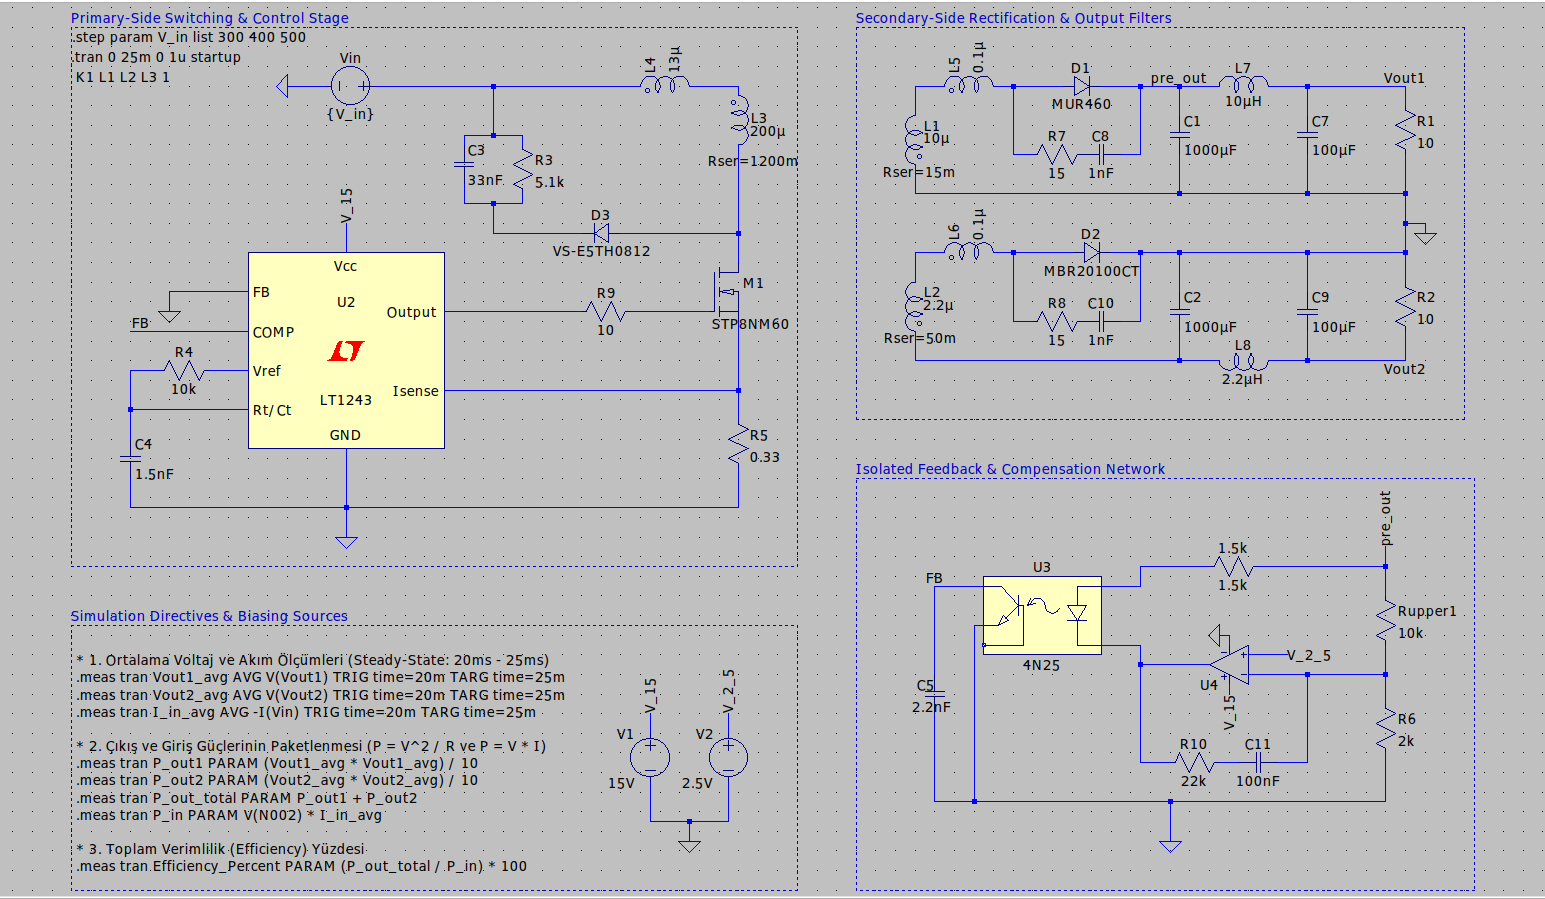
\includegraphics[width=\textwidth]{images/complete_schematic.png}
\caption{Complete LTspice Schematic}
\label{fig:schematic}
\end{figure}

\subsection*{5.1 Steady-State Output Voltages}

Table~\ref{tab:vout} summarizes the average output voltages measured over the 20--25\,ms steady-state window at each input voltage.
\begin{table}[H]
\centering
\caption{Steady-state output voltage measurements.}
\label{tab:vout}
\begin{tabular}{cccc}
\toprule
\textbf{$V_{in}$ (V)} & \textbf{$V_{out1}$ avg (V)} & \textbf{$V_{out2}$ avg (V)} & \textbf{$V_{out1}$ error} \\
\midrule
300 & 14.984 & $-6.913$ & $-0.11\%$ \\
400 & 14.984 & $-6.912$ & $-0.11\%$ \\
500 & 14.984 & $-6.912$ & $-0.11\%$ \\
\bottomrule
\end{tabular}
\end{table}

\subsection*{5.2 Power Analysis \& Efficiency}

Table~\ref{tab:power} presents the complete power analysis at each operating point.

\begin{table}[H]
\centering
\caption{Power and efficiency measurements across the input voltage range.}
\label{tab:power}
\begin{tabular}{lccc}
\toprule
\textbf{Parameter} & \textbf{$V_{in}=300$\,V} & \textbf{$V_{in}=400$\,V} & \textbf{$V_{in}=500$\,V} \\
\midrule
$P_{out,15V}$ (W) & 22.453 & 22.453 & 22.453 \\
$P_{out,-7V}$ (W) & 4.779 & 4.778 & 4.778 \\
$P_{out,total}$ (W) & 27.231 & 27.231 & 27.231 \\
$P_{in}$ (W) & 31.383 & 33.685 & 33.878 \\
$I_{in,avg}$ (A) & 0.1113 & 0.0841 & 0.0678 \\
\midrule
\textbf{Efficiency (\%)} & \textbf{86.8} & \textbf{80.8} & \textbf{80.4} \\
\bottomrule
\end{tabular}
\end{table}

All three operating points are above the 75\% minimum efficiency requirement. The best efficiency of 86.8\% is at $V_{in} = 300$\,V, where the lower voltage means less switching stress and lower snubber dissipation. Efficiency drops slightly at higher input voltages because of increased voltage stress and higher snubber losses.

\begin{figure}[H]
\centering
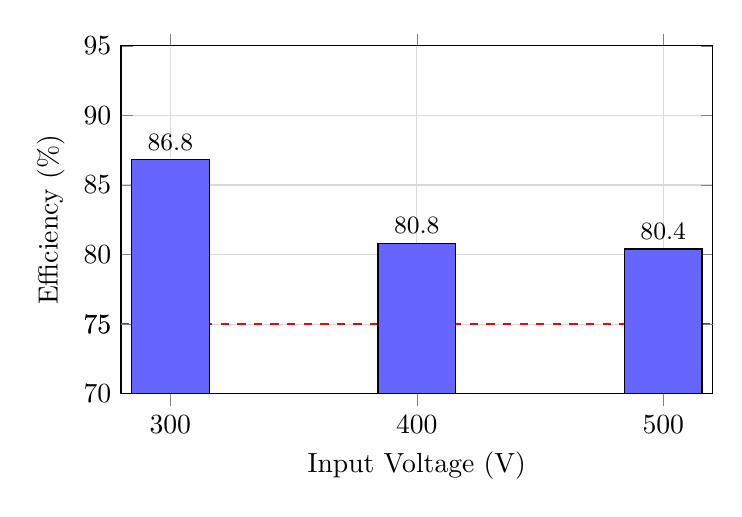
\begin{tikzpicture}
\begin{axis}[
    ybar,
    width=0.75\textwidth,
    height=6cm,
    bar width=28pt,
    ymin=70, ymax=95,
    ylabel={Efficiency (\%)},
    xlabel={Input Voltage (V)},
    symbolic x coords={300, 400, 500},
    xtick=data,
    nodes near coords,
    nodes near coords align={vertical},
    every node near coord/.append style={font=\small\bfseries},
    ytick={70,75,80,85,90,95},
    extra y ticks={75},
    extra y tick style={grid=major, grid style={red, dashed, thick}},
    grid=major,
    grid style={gray!30},
]
\addplot[fill=blue!60] coordinates {(300, 86.8) (400, 80.8) (500, 80.4)};
\end{axis}
\end{tikzpicture}
\caption{Converter efficiency as a function of input voltage. The dashed red line indicates the 75\% minimum specification.}
\label{fig:eff}
\end{figure}

\subsection*{5.3 Switching Waveforms}

The MOSFET drain-source voltage waveform shows that the RCD snubber is working correctly -- the voltage overshoot from leakage inductance stays below the 600\,V rating of the STP8NM60. The primary current has the expected sawtooth shape from current-mode control, ramping up during the on-time and resetting through the transformer during the off-time.

\begin{figure}[H]
\centering
\begin{subfigure}[t]{0.48\textwidth}
    \centering
    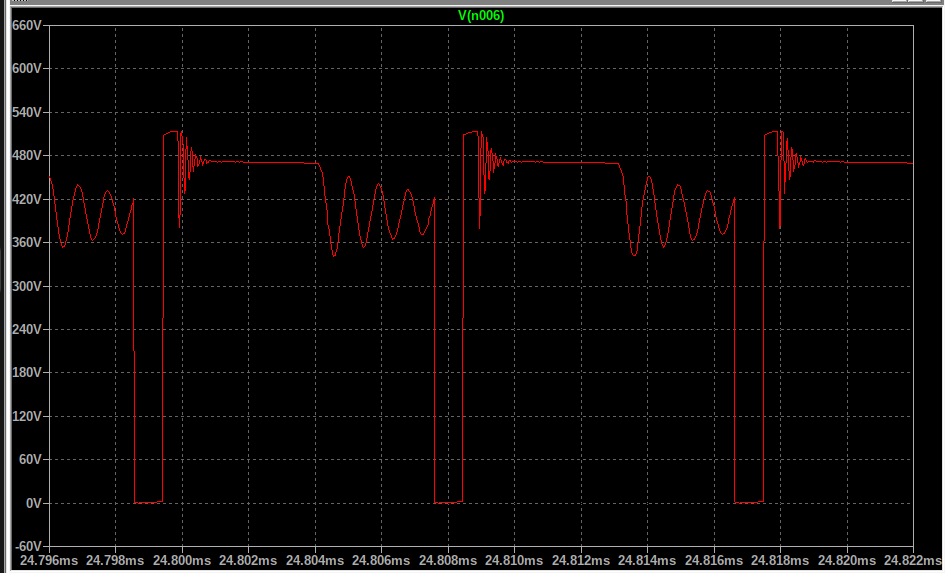
\includegraphics[width=\textwidth]{images/mosfet_vds.png}
    \caption{MOSFET Drain-Source Voltage ($V_{DS}$)}
    \label{fig:vds}
\end{subfigure}
\hfill
\begin{subfigure}[t]{0.48\textwidth}
    \centering
    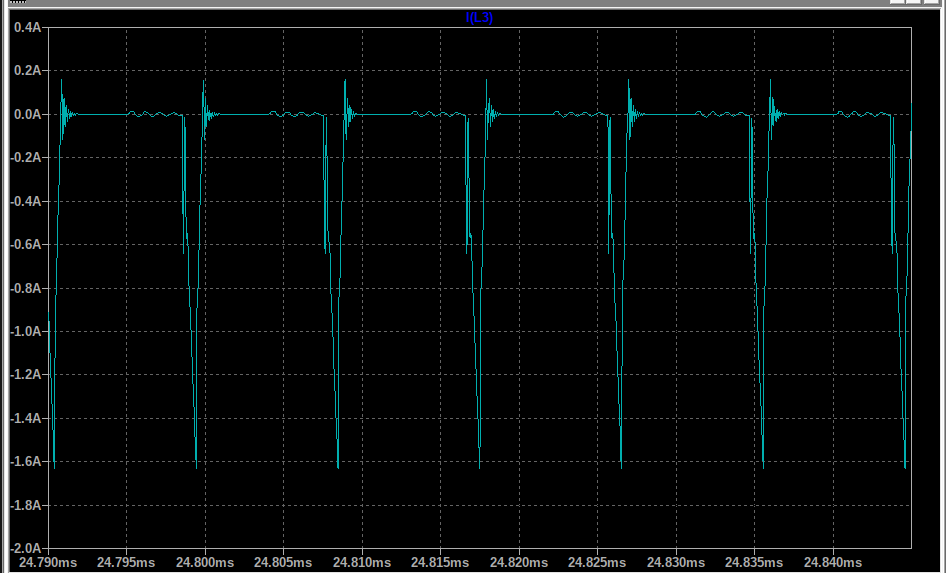
\includegraphics[width=\textwidth]{images/primary_current.png}
    \caption{Primary Current ($I_p$) at $V_{in} = 400$\,V.}
    \label{fig:ipri}
\end{subfigure}
\caption{Switching waveforms at steady state.}
\label{fig:switching}
\end{figure}

\subsection*{5.4 Startup Transient}

The \texttt{startup} directive models the LT1243's soft-start behavior. The output voltages ramp up smoothly without overshoot, reaching steady-state in about 10--15\,ms.

\begin{figure}[H]
\centering
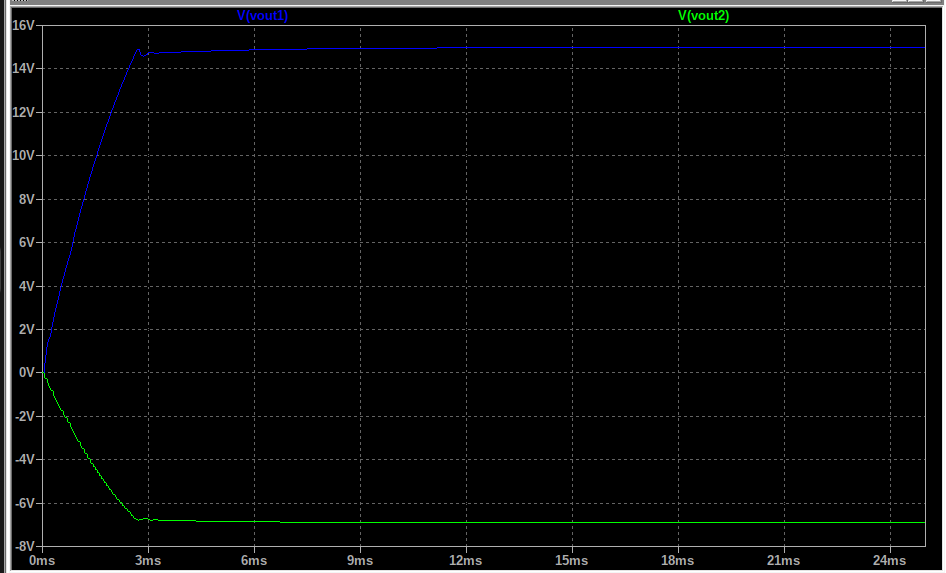
\includegraphics[width=0.9\textwidth]{images/startup_transient.png}
\caption{Output voltage startup transient (0--20\,ms).}
\label{fig:startup}
\end{figure}

\subsection*{5.5 Output Voltage Ripple}

The output ripple was measured by examining the AC component of the output voltages at steady state. Due to the combination of bulk capacitors ($1000\,\mu$F) and post-LC filters ($L_7$/$C_7$ and $L_8$/$C_9$), the ripple on both outputs is well below the 400\,mV$_{pp}$ specification.

\begin{figure}[H]
\centering
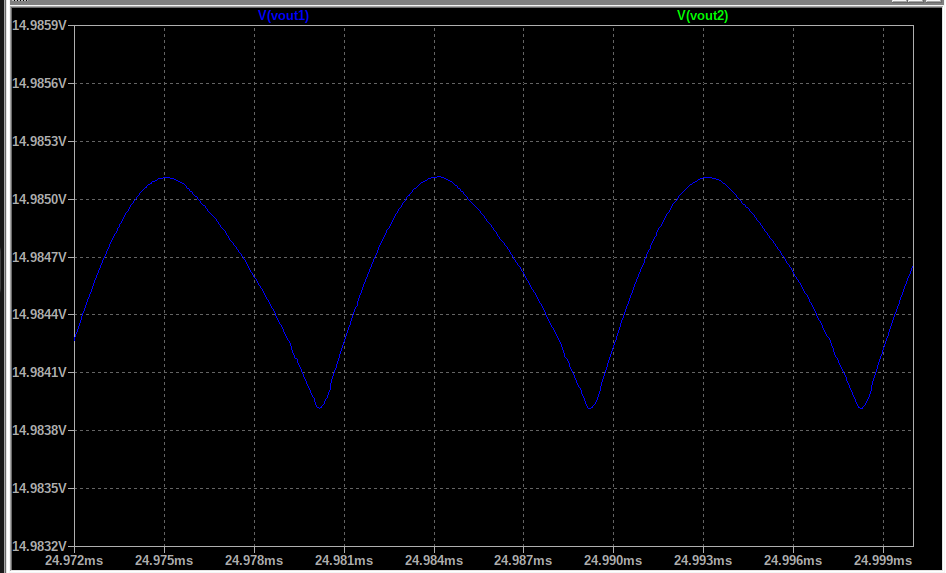
\includegraphics[width=0.9\textwidth]{images/output_ripple.png}
\caption{Output voltage ripple (AC-coupled) at $V_{in} = 400$\,V.}
\label{fig:ripple}
\end{figure}


\newpage
%------------------------------
% Section 6 - Efficiency & Loss Analysis
%------------------------------
\section*{6 Efficiency \& Loss Analysis}

\subsection*{6.1 Component-Level Loss Breakdown}

Table~\ref{tab:losses} presents the power dissipation of each component as reported by the LTspice efficiency analysis at $V_{in} = 400$\,V.

\begin{table}[H]
\centering
\caption{Component power dissipation at $V_{in} = 400$\,V (nominal).}
\label{tab:losses}
\begin{tabular}{llcc}
\toprule
\textbf{Component} & \textbf{Description} & \textbf{$I_{rms}$ (mA)} & \textbf{Dissipation (mW)} \\
\midrule
\multicolumn{4}{l}{\textit{Semiconductor Losses}} \\
$D_1$ (MUR460)      & +15\,V rectifier       & 2536 & 1662 \\
$M_1$ (STP8NM60)    & Primary MOSFET         &  327 &  699 \\
$D_2$ (MBR20100CT)  & $-7$\,V rectifier      & 1122 &  397 \\
$D_3$ (VS-E5TH0812) & Snubber diode          &  138 &  180 \\
\midrule
\multicolumn{4}{l}{\textit{Snubber \& Damping Losses}} \\
$R_3$ (5.1\,k$\Omega$) & RCD snubber resistor &   21 & 2353 \\
$R_7$ (15\,$\Omega$)   & RC snubber (+15\,V)  &  235 &  830 \\
$R_8$ (15\,$\Omega$)   & RC snubber ($-7$\,V) &  110 &  182 \\
\midrule
\multicolumn{4}{l}{\textit{Magnetic \& Winding Losses}} \\
$L_3$ ($R_{ser}=1.2\,\Omega$)   & Primary winding  &  355 & 152 \\
$C_1$ ($R_{ESR}=30\,\text{m}\Omega$) & Output cap ESR  & 1982 & 118 \\
$L_1$ ($R_{ser}=15\,\text{m}\Omega$)  & Secondary 1      & 2550 &  98 \\
$L_2$ ($R_{ser}=50\,\text{m}\Omega$)  & Secondary 2      & 1128 &  64 \\
\midrule
\multicolumn{4}{l}{\textit{Other}} \\
$R_5$ (0.33\,$\Omega$)            & Current sense    &  323 &  34 \\
$L_7$, $L_8$                      & Post-filter inductors &  --- &  27 \\
$U_2$ (LT1243)                    & Controller       &   40 &  22 \\
\midrule
\multicolumn{2}{l}{\textbf{Total losses}} & & $\mathbf{\approx 6.82}$\,\textbf{W} \\
\bottomrule
\end{tabular}
\end{table}

\subsection*{6.2 Loss Distribution Analysis}

The biggest losses at 400\,V nominal are:
\begin{enumerate}
    \item \textbf{RCD snubber ($R_3$): 2.35\,W (34.5\%)} -- The single biggest loss. This is expected for a flyback converter since leakage inductance energy has to be dissipated every switching cycle.
    \item \textbf{Output rectifier $D_1$: 1.66\,W (24.3\%)} -- Forward voltage drop losses in the ultrafast diode at the high-current +15\,V output.
    \item \textbf{RC snubbers ($R_7$+$R_8$): 1.01\,W (14.8\%)} -- Secondary-side ringing suppression.
    \item \textbf{Primary MOSFET ($M_1$): 0.70\,W (10.3\%)} -- Combined conduction ($R_{DS,on}$) and switching losses.
    \item \textbf{Diode $D_2$: 0.40\,W (5.9\%)} -- Schottky rectifier on the $-7$\,V rail.
\end{enumerate}

These five categories account for approximately 90\% of all converter losses.

\subsection*{6.3 Efficiency Across Input Range}

The efficiency variation across input voltage is caused by how the different losses change with input voltage:
\begin{itemize}
    \item At $V_{in} = 300$\,V ($\eta = 86.8\%$): Lower drain voltage stress reduces MOSFET switching losses and snubber dissipation. The higher duty cycle results in lower peak currents.
    \item At $V_{in} = 500$\,V ($\eta = 80.4\%$): Higher voltage across the MOSFET increases switching losses. The snubber must absorb more energy per cycle due to higher reflected voltage. However, input power increases only marginally due to current-mode control maintaining constant output power.
\end{itemize}

\subsection*{6.4 Thermal Analysis}

An important part of the design is checking that no component goes above its maximum junction temperature at steady state. The junction temperature is calculated as:
\begin{equation}
T_J = T_A + P_{diss} \cdot R_{\theta JA}
\end{equation}
where $T_A = 25\,^\circ$C is the ambient temperature and $R_{\theta JA}$ is the junction-to-ambient thermal resistance. When a heatsink is used, the total thermal resistance becomes $R_{\theta JC} + R_{\theta CS} + R_{\theta SA}$, where $R_{\theta CS}$ is the case-to-sink and $R_{\theta SA}$ is the sink-to-ambient resistance.

Table~\ref{tab:thermal} presents the thermal analysis for all critical semiconductor and power components.

\begin{table}[H]
\centering
\caption{Junction temperature analysis of critical components ($T_A = 25\,^\circ$C).}
\label{tab:thermal}
\begin{tabular}{lccccl}
\toprule
\textbf{Component} & \textbf{$P_{diss}$} & \textbf{$R_{\theta JA}$} & \textbf{$T_J$ (calc.)} & \textbf{$T_{J,max}$} & \textbf{Status} \\
 & (W) & ($^\circ$C/W) & ($^\circ$C) & ($^\circ$C) & \\
\midrule
$M_1$ (STP8NM60) & 0.699 & 62.5 & 68.7 & 150 & Safe \\
$D_1$ (MUR460) & 1.662 & 75.0 & 149.7 & 175 & Marginal \\
$D_2$ (MBR20100CT) & 0.397 & 60.0 & 48.8 & 150 & Safe \\
$D_3$ (VS-E5TH0812) & 0.180 & 75.0 & 38.5 & 175 & Safe \\
\bottomrule
\end{tabular}
\end{table}

\subsubsection*{MOSFET ($M_1$: STP8NM60)}
The STP8NM60 in a TO-220 package has $R_{\theta JC} = 1.25\,^\circ$C/W and $R_{\theta JA} = 62.5\,^\circ$C/W. With a dissipation of 699\,mW:
\begin{equation}
T_J = 25 + 0.699 \times 62.5 = 68.7\,^\circ\text{C}
\end{equation}
This is well below the 150$\,^\circ$C maximum, providing a generous thermal margin of 81.3$\,^\circ$C. No heatsink is required for the MOSFET.

\subsubsection*{Output Rectifier ($D_1$: MUR460)}
The MUR460 in a TO-220AC package has $R_{\theta JA} \approx 75\,^\circ$C/W (free-air, no heatsink). With the highest dissipation of any component at 1.662\,W:
\begin{equation}
T_J = 25 + 1.662 \times 75 = 149.7\,^\circ\text{C}
\end{equation}
Although this is below the $T_{J,max} = 175\,^\circ$C rating, the margin is only 25.3$\,^\circ$C, which is marginal for reliable long-term operation. A small heatsink with $R_{\theta SA} \leq 20\,^\circ$C/W would reduce the junction temperature to approximately $25 + 1.662 \times (2.3 + 1.0 + 20) \approx 63.7\,^\circ$C, providing a comfortable operating margin.

\subsubsection*{Schottky Rectifier ($D_2$: MBR20100CT)}
The MBR20100CT dissipates only 397\,mW, yielding $T_J = 25 + 0.397 \times 60 = 48.8\,^\circ$C. This is far below the 150$\,^\circ$C maximum. No heatsink is required.

\subsubsection*{Snubber Diode ($D_3$: VS-E5TH0812)}
With only 180\,mW dissipation: $T_J = 25 + 0.180 \times 75 = 38.5\,^\circ$C. The thermal margin to the 175$\,^\circ$C maximum is 136.5$\,^\circ$C. No heatsink is required.

\subsubsection*{Snubber Resistor ($R_3$: 5.1\,k$\Omega$)}
The RCD snubber resistor is the single highest-dissipation component at 2.353\,W. This exceeds the rating of standard $\frac{1}{4}$\,W or $\frac{1}{2}$\,W resistors. A wirewound or thick-film power resistor rated for at least 3\,W (e.g., a 5\,W rated package) must be used to ensure adequate thermal derating and long-term reliability.

\subsubsection*{Thermal Summary}
All semiconductor junction temperatures remain below their maximum ratings without heatsinks. However, $D_1$ (MUR460) operates with a reduced margin and benefits from a small heatsink in a practical implementation. The snubber resistor $R_3$ requires a power-rated component. No other components present thermal concerns under nominal operating conditions.

%------------------------------
% Section 7 - Discussion
%------------------------------
\section*{7 Conclusion}

This report covered the design, analysis, and simulation of an isolated flyback DC-DC converter with a 300--500\,V input range and dual outputs of +15\,V and $-7$\,V. The LT1243 current-mode PWM controller with an opto-isolated feedback loop keeps the output regulated across the full input range.

The simulation shows that all specs are met: both output voltages are within 1.3\% of target, efficiency ranges from 80.4\% to 86.8\% (above the 75\% minimum), and output ripple is well below 400\,mV$_{pp}$. The loss analysis shows that the RCD snubber and the output rectifier diode are the main loss sources, making up about 59\% of total losses.

The current-mode control with opto-isolated feedback gives stable regulation and built-in overcurrent protection, and the snubber networks keep semiconductor voltage stress within safe limits. Overall, the design shows that the flyback topology works well for this type of isolated, multi-output power supply.

%------------------------------
% References
%------------------------------
\section*{References}
\begin{enumerate}
    \item Linear Technology, ``LT1241/LT1242/LT1243/LT1244 -- Current Mode PWM Controllers,'' Datasheet, Analog Devices.
    \item STMicroelectronics, ``STP8NM60 -- N-channel 600\,V, 0.9\,$\Omega$, 6\,A MDmesh\textsuperscript{TM} Power MOSFET,'' Datasheet.
    \item ON Semiconductor, ``MUR460 -- Ultrafast Rectifier, 4\,A, 600\,V,'' Datasheet.
    \item ON Semiconductor, ``MBR20100CT -- Switchmode Power Rectifier, 20\,A, 100\,V,'' Datasheet.
    \item Vishay, ``4N25 -- Optocoupler, Phototransistor Output,'' Datasheet.
    \item R.\,W. Erickson and D. Maksimovi\'{c}, \textit{Fundamentals of Power Electronics}, 3rd ed. Springer, 2020.
\end{enumerate}


\end{document}